\documentclass{beamer}\usepackage[]{graphicx}\usepackage[]{color}
%% maxwidth is the original width if it is less than linewidth
%% otherwise use linewidth (to make sure the graphics do not exceed the margin)
\makeatletter
\def\maxwidth{ %
  \ifdim\Gin@nat@width>\linewidth
    \linewidth
  \else
    \Gin@nat@width
  \fi
}
\makeatother

\definecolor{fgcolor}{rgb}{0.345, 0.345, 0.345}
\newcommand{\hlnum}[1]{\textcolor[rgb]{0.686,0.059,0.569}{#1}}%
\newcommand{\hlstr}[1]{\textcolor[rgb]{0.192,0.494,0.8}{#1}}%
\newcommand{\hlcom}[1]{\textcolor[rgb]{0.678,0.584,0.686}{\textit{#1}}}%
\newcommand{\hlopt}[1]{\textcolor[rgb]{0,0,0}{#1}}%
\newcommand{\hlstd}[1]{\textcolor[rgb]{0.345,0.345,0.345}{#1}}%
\newcommand{\hlkwa}[1]{\textcolor[rgb]{0.161,0.373,0.58}{\textbf{#1}}}%
\newcommand{\hlkwb}[1]{\textcolor[rgb]{0.69,0.353,0.396}{#1}}%
\newcommand{\hlkwc}[1]{\textcolor[rgb]{0.333,0.667,0.333}{#1}}%
\newcommand{\hlkwd}[1]{\textcolor[rgb]{0.737,0.353,0.396}{\textbf{#1}}}%
\let\hlipl\hlkwb

\usepackage{framed}
\makeatletter
\newenvironment{kframe}{%
 \def\at@end@of@kframe{}%
 \ifinner\ifhmode%
  \def\at@end@of@kframe{\end{minipage}}%
  \begin{minipage}{\columnwidth}%
 \fi\fi%
 \def\FrameCommand##1{\hskip\@totalleftmargin \hskip-\fboxsep
 \colorbox{shadecolor}{##1}\hskip-\fboxsep
     % There is no \\@totalrightmargin, so:
     \hskip-\linewidth \hskip-\@totalleftmargin \hskip\columnwidth}%
 \MakeFramed {\advance\hsize-\width
   \@totalleftmargin\z@ \linewidth\hsize
   \@setminipage}}%
 {\par\unskip\endMakeFramed%
 \at@end@of@kframe}
\makeatother

\definecolor{shadecolor}{rgb}{.97, .97, .97}
\definecolor{messagecolor}{rgb}{0, 0, 0}
\definecolor{warningcolor}{rgb}{1, 0, 1}
\definecolor{errorcolor}{rgb}{1, 0, 0}
\newenvironment{knitrout}{}{} % an empty environment to be redefined in TeX

\usepackage{alltt}
\usetheme{}
\usecolortheme{}
\IfFileExists{upquote.sty}{\usepackage{upquote}}{}
\begin{document}

\title{Wordcloud with Sentiments: Alice in Wonderland}
\author{Judy Minichelli}

\begin{frame}
  \titlepage
\end{frame}

\begin{frame}[fragile]
  \frametitle{Outline}
   \tableofcontents
\end{frame}

\section{Install and load libraries}
\begin{frame}[fragile]
  \frametitle{Install and load libraries}
   \begin{itemize}
    \item<1->
\begin{knitrout}
\definecolor{shadecolor}{rgb}{0.969, 0.969, 0.969}\color{fgcolor}\begin{kframe}
\begin{alltt}
\hlkwd{library}\hlstd{(dplyr)}
\end{alltt}
\end{kframe}
\end{knitrout}
     \item<2->
\begin{knitrout}
\definecolor{shadecolor}{rgb}{0.969, 0.969, 0.969}\color{fgcolor}\begin{kframe}
\begin{alltt}
\hlkwd{library}\hlstd{(ggplot2)}
\end{alltt}
\end{kframe}
\end{knitrout}
     \item<3->
\begin{knitrout}
\definecolor{shadecolor}{rgb}{0.969, 0.969, 0.969}\color{fgcolor}\begin{kframe}
\begin{alltt}
\hlkwd{library}\hlstd{(gutenbergr)}
\end{alltt}
\end{kframe}
\end{knitrout}
     \item<4->
\begin{knitrout}
\definecolor{shadecolor}{rgb}{0.969, 0.969, 0.969}\color{fgcolor}\begin{kframe}
\begin{alltt}
\hlkwd{library}\hlstd{(stringr)}
\end{alltt}
\end{kframe}
\end{knitrout}
     \item<5->  
\begin{knitrout}
\definecolor{shadecolor}{rgb}{0.969, 0.969, 0.969}\color{fgcolor}\begin{kframe}
\begin{alltt}
\hlkwd{library}\hlstd{(tidytext)}
\end{alltt}
\end{kframe}
\end{knitrout}
     \item<6->  
\begin{knitrout}
\definecolor{shadecolor}{rgb}{0.969, 0.969, 0.969}\color{fgcolor}\begin{kframe}
\begin{alltt}
\hlkwd{library}\hlstd{(wordcloud)}
\end{alltt}
\end{kframe}
\end{knitrout}
     \item<7->  
\begin{knitrout}
\definecolor{shadecolor}{rgb}{0.969, 0.969, 0.969}\color{fgcolor}\begin{kframe}
\begin{alltt}
\hlkwd{library}\hlstd{(wordcloud2)}
\end{alltt}
\end{kframe}
\end{knitrout}
     \item<8->  
\begin{knitrout}
\definecolor{shadecolor}{rgb}{0.969, 0.969, 0.969}\color{fgcolor}\begin{kframe}
\begin{alltt}
\hlkwd{library}\hlstd{(reshape2)}
\end{alltt}
\end{kframe}
\end{knitrout}
    
    \end{itemize}
\end{frame}

\section{Download Alice in Wonderland text}
\begin{frame}[fragile]
 \frametitle{Download Alice in Wonderland text}
\begin{knitrout}
\definecolor{shadecolor}{rgb}{0.969, 0.969, 0.969}\color{fgcolor}\begin{kframe}
\begin{alltt}
\hlstd{alice}\hlkwb{<-}\hlkwd{gutenberg_download}\hlstd{(}\hlnum{11}\hlstd{)}
\end{alltt}
\end{kframe}
\end{knitrout}
\end{frame}

%%Showing 500th line of the text.  498:500 would be those 3 lines.  %%Substring is pulling out first 21 characters of the those lines %%because they are too long.

\section{Remove Chapter Headings}
 \begin{frame}[fragile]
  \frametitle{Remove Chapter Headings}
\begin{knitrout}
\definecolor{shadecolor}{rgb}{0.969, 0.969, 0.969}\color{fgcolor}\begin{kframe}
\begin{alltt}
\hlstd{alice}\hlkwb{<-}\hlstd{alice}\hlopt
\hlkwd{filter}\hlstd{(}\hlopt{!}\hlkwd{str_detect}\hlstd{(alice}\hlopt{$}\hlstd{text,}\hlstr{'^CHAPTER'}\hlstd{))}

\hlstd{alice}\hlkwb{<-}\hlstd{alice[}\hlnum{10}\hlopt{:}\hlnum{3339}\hlstd{,]}
\end{alltt}
\end{kframe}
\end{knitrout}
\end{frame}

\section{Unpack the Words}
 \begin{frame}[fragile]
  \frametitle{Unpack the Words}
\begin{knitrout}
\definecolor{shadecolor}{rgb}{0.969, 0.969, 0.969}\color{fgcolor}\begin{kframe}
\begin{alltt}
\hlstd{alice_words}\hlkwb{<-}\hlstd{alice}\hlopt
\hlkwd{unnest_tokens}\hlstd{(word,text)}
\end{alltt}
\end{kframe}
\end{knitrout}
\end{frame}

\section{The Bing Lexicon}
 \begin{frame}[fragile]
  \frametitle{The Bing Lexicon}
\begin{knitrout}
\definecolor{shadecolor}{rgb}{0.969, 0.969, 0.969}\color{fgcolor}\begin{kframe}
\begin{alltt}
   \hlstd{bing}\hlkwb{<-}\hlkwd{get_sentiments}\hlstd{(}\hlstr{'bing'}\hlstd{)}
\end{alltt}
\end{kframe}
\end{knitrout}
\end{frame}

\section{The Inner Join}
 \begin{frame}[fragile]
  \frametitle{The Inner Join}
\begin{knitrout}
\definecolor{shadecolor}{rgb}{0.969, 0.969, 0.969}\color{fgcolor}\begin{kframe}
\begin{alltt}
\hlstd{alice_words}\hlkwb{<-}\hlkwd{inner_join}\hlstd{(alice_words,bing)}
\hlstd{alice_words}\hlopt{$}\hlstd{gutenberg_id}\hlkwb{<-}\hlkwa{NULL}
\end{alltt}
\end{kframe}
\end{knitrout}
\end{frame}

\section{Assign Sentiments}
 \begin{frame}[fragile,allowframebreaks]
  \frametitle{Assign Sentiments}
\begin{knitrout}
\definecolor{shadecolor}{rgb}{0.969, 0.969, 0.969}\color{fgcolor}\begin{kframe}
\begin{alltt}
  \hlstd{alice_words}\hlkwb{<-}\hlstd{alice_words}\hlopt
  \hlkwd{group_by}\hlstd{(word)}\hlopt
  \hlkwd{summarize}\hlstd{(}\hlkwc{freq}\hlstd{=}\hlkwd{n}\hlstd{(),}\hlkwc{sentiment}\hlstd{=}\hlkwd{first}\hlstd{(sentiment))}
\end{alltt}
\end{kframe}
\end{knitrout}
\end{frame}

\section{Wordcloud}
 \begin{frame}[fragile,allowframebreaks]
  \frametitle{Wordcloud}
\begin{knitrout}
\definecolor{shadecolor}{rgb}{0.969, 0.969, 0.969}\color{fgcolor}\begin{kframe}
\begin{alltt}
\hlkwd{wordcloud}\hlstd{(alice_words}\hlopt{$}\hlstd{word,alice_words}\hlopt{$}\hlstd{freq,} \hlkwc{min.freq} \hlstd{=} \hlnum{3}\hlstd{)}
\end{alltt}
\end{kframe}
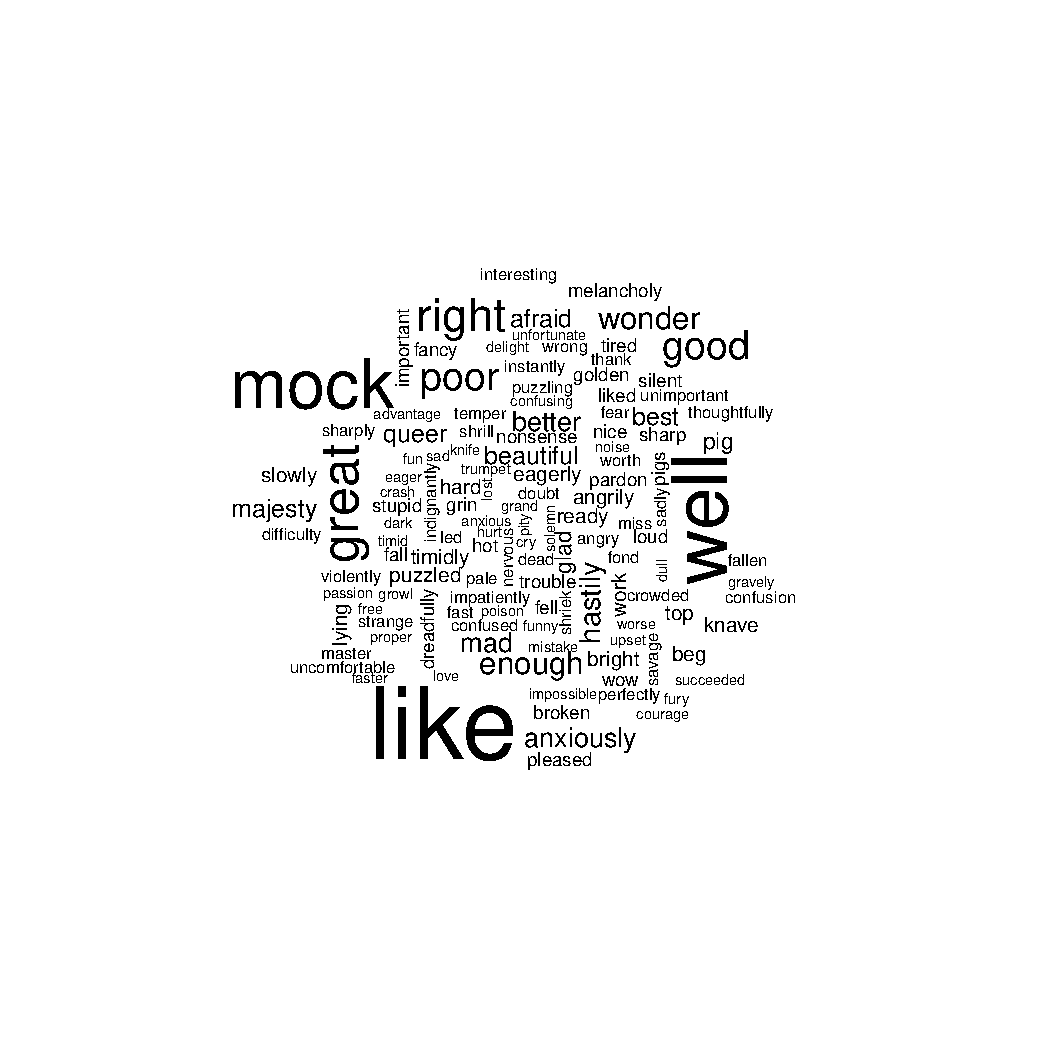
\includegraphics[width=\maxwidth]{figure/unnamed-chunk-15-1} 

\end{knitrout}
\end{frame}

\section{Distinguish between Positive from Negative Sentiments}
 \begin{frame}[fragile,allowframebreaks]
  \frametitle{Distinguish between Positive from Negative Sentiments}
\begin{knitrout}
\definecolor{shadecolor}{rgb}{0.969, 0.969, 0.969}\color{fgcolor}\begin{kframe}
\begin{alltt}
\hlcom{#alice_matrix<-acast(alice_words,word~sentiment,}
                    \hlcom{#value.var='freq',fill=0)}
\hlcom{#comparison.cloud(alice_matrix,colors=c('red','green'))}

\hlcom{#Using .png "rplot" below instead of actual plot from code }
\hlcom{#so the whole figure is visible on the slide (Heidi's idea)}
\end{alltt}
\end{kframe}
\end{knitrout}

\begin{figure}
\includegraphics[scale=0.5]{rplot}
\end{figure}

\end{frame}

\end{document}
